\documentclass{report}

% Language setting
% Replace `english' with e.g. `spanish' to change the document language
\usepackage[serbian]{babel}

% Set page size and margins
% Replace `letterpaper' with `a4paper' for UK/EU standard size
\usepackage[letterpaper,top=2cm,bottom=2cm,left=3cm,right=3cm,marginparwidth=1.75cm]{geometry}

% Useful packages
\usepackage{amsmath}
\usepackage{graphicx}
\usepackage[colorlinks=true, allcolors=blue]{hyperref}
\newcommand{\HRule}{\rule{\linewidth}{0.5mm}}

\begin{document}
%\title{}
\vspace*{5cm}
\thispagestyle{empty}
\centerline{\huge \textbf{MATEMATIČKI FAKULTET}}
\vspace{2cm}

\begin{center}

{\Large Seminarski rad}\\
{\Large	iz Tehničkog i naučnog pisanja}\\
\Huge\HRule\\[0.4cm] %0.4cm
	{Robotika u 2022.}\\
	\HRule \\[20pt] %20pt
\begin{minipage}{0.4\textwidth}
\begin{flushleft} \large
{\Large Luka Matić}\\
{\Large Marko Cvijetinović}
\end{flushleft}
\end{minipage}
~
\begin{minipage}{0.4\textwidth}
\begin{flushright} \large
{\Large Đuro Cerović} \\
{\Large Mihajlo Radojević}\\ 
\end{flushright}
\end{minipage}\\[5cm]
\Large{Beograd, Novembar 2022.}
\end{center}

%\begin{abstract}
%bbla blablaf
%\end{abstract}
\tableofcontents
\chapter{Saradnički roboti}

Usled restrikcija postavljenih zbog COVID-19 pandemije, dolazi do sve veće potražnje za robotima koji bi komplementirali rad zaposlenih. Toliko, da popularnost saradničkih robota dovodi do nestajanja strepnji kako će roboti preuzeti poslove ljudima. Realnost je da oni pomažu ljudima da rade lakše i bezbednije dok riboti preuzimaju mesta nepoželjna za ljude.

Za razliku od konvencionalnih, saradnički roboti su dizajnirani da rade sa ljudima, a ne u izolaciji. Ovo omogućava kompanijama da kombinuju prednosti ljudi i robota, što povećava produktivnost. \cite{robotics2022}

Saradnički roboti mogu da rade suvoparne, prljave i opasne poslove koje su nekad izvršavali ljudi. To može biti od nezamisljive važnosti u državamsa sa većinski fakultetski obrazovanim stanovništvom, jer oni ne žele da se bave takvim poslovim pa dolazi do manjka radne snage.

Pokrivanjem radnih mesta na nižem nivou, saradnički roboti omogućavaju ljudima da okupiraju više funkcije u kompanijama. Ne samo da ovo ide u korist radnicima, već je moguće i doći do veće efikasnosti i preciznosti jer automatizovana tehnologija nije sklona pravljenju grešaka kao ljudi.

Povrh svega toga, roboti mogu da rade bez prestanka što očigledno povećava prihode, a i olakšava izvršavanje poslova zadatih u kratkom vremenskom roku. \cite{cobots}

\begin{figure}
\centering
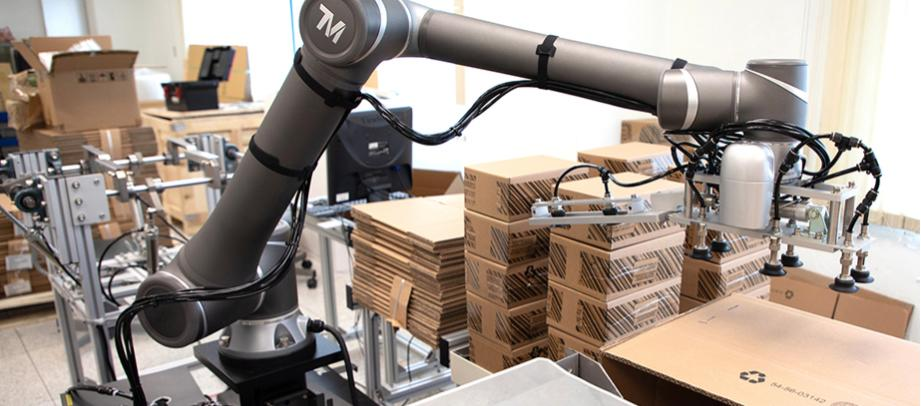
\includegraphics[scale=0.41]{Cobot.jpg}
\caption{Saradnički roboti često rade u fabrikama, pakuju, raspakuju ili razmeštaju objekte (Slika preuzeta sa https://kinemarobotica.com.).}
\end{figure}

\chapter{Roboti dostavljači}
Slično kao i saradnički roboti, ovaj trend je nastao usled COVID-19 epidemije zarad smanjenja kontakta između zaposlenih i mušterija jer to može dovesti do širenja zaraze.

Automatizovana dostava hrane i ostalih manjih porudžbina je dostigla toliku popularnost za svega godinu ili dve, da neke Američke države već imaju zakone koje regulišu gde roboti dostavljači smeju da se kreću. Još jedna prednost robota u ovom poslu je fleksibilnost i u stanju su da obave i one porudžbine čija je isporuka zahtevana istog dana.
\vspace{0.25cm}
\begin{center}
\begin{tabular}{ |p{1cm}|p{1cm}|p{1cm}|p{1cm} |p{1cm}|p{1cm}|p{1cm}|p{1cm}|p{1cm}|p{1cm}|p{1cm}|}
\hline
\multicolumn{11}{|c|}{Procenat isporuka koji je stigao u obećano vreme u SAD-u po mesecima} \\
\hline
Godina & Mart & April & Maj & Jun & Jul & Avgust & Sept. & Okt. & Nov. & Dec. \\
\hline
2019 & 88 & 89 & 89 & 89 & 89 & 89 & 87 & 88 & 86 & 75 \\
2020 & 85 & 76 & 72 & 71 & 77 & 77 & 80 & 82 & 80 & 72 \\
\hline
\end{tabular}
\end{center}
\vspace{0.25cm}
Zabeležava se rast broja porudžbina i smanjenje traženog roka isporuke iz godine u godinu, što doprinosi povećanju potražnje robota za dostavu. \cite{robotics2022, sameday}  

\chapter{Prediktivno održavanje}
Robotika može da uštedi ogromne količine novca tokom vremena, ali takođe dolazi sa troškovima održavanja kako bi se obezbedile vrhunske performanse. Kao rezultat, prediktivno održavanje je u porastu u robotici ove godine. Prediktivno održavanje koristi tehnologiju kao što su senzori Interneta stvari za praćenje performansi i fizičkog stanja robota. Podaci senzora otkrivaju pad performansi koji ukazuje kada je vreme da se završi održavanje pre nego što je potrebna velika popravka.

IoT senzori su takođe korisni u robotskoj automatizaciji procesa, gde mogu da pomognu u vođenju robota u veoma korisnim zadacima, kao što je kontrola kvaliteta. IoT i tehnologije daljinskog otkrivanja i praćenja postaju posebno popularne u skladištima, gde se roboti koriste za sve, od sakupljanja artikala sa polica do pakovanja kutija za otpremu.
 \cite{robotic2022}


\centering
\vspace{2cm}
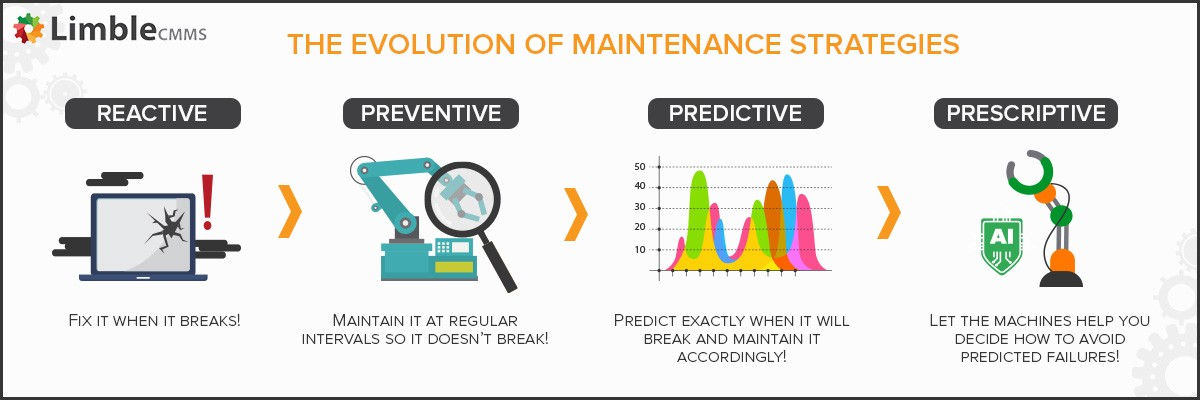
\includegraphics[scale=0.37]{dijagram.jpeg}
Prediktivno održavanje se odnosi na upotrebu proaktivnih metoda održavanja zasnovanih na podacima koje su dizajnirane da analiziraju stanje opreme i pomažu u predviđanju kada održavanje treba da se izvrši. (Slika preuzeta sa \url{https://www.heavy.ai/technical-glossary/predictive-maintenance}).

\chapter{Povećanje kompatibilnosti}
Sa toliko usvajanja i inovacija u robotici, raznovrsnost i prilagođavanje postaju briga za neka preduzeća. U 2022. sve više programera robotike ima to na umu. Industrijski stručnjaci su istakli
\href{https://enterprisersproject.com/article/2022/1/4-robotic-process-automation-rpa-trends-watch-2022}{trend ka saradnji}.u RPA ove godine, uz napomenu da se oslanja na kombinovanje brojnih tehnologija za maksimalnu efikasnost.
Ovaj trend obuhvata AI i mašinsko učenje, ali i druge robote. Proizvodnoj kompaniji, na primer, mogu biti potrebni potpuno različiti roboti za različite delove svog proizvodnog procesa ili za pravljenje različitih proizvoda. Postaje tržišna prednost za robote da budu lako kompatibilni sa drugim, potpuno drugačijim robotima. Ovo je zanimljiv kontrast u odnosu na druge industrije, ali ukazuje na budućnost koja se oslanja na robote.
 \cite{robot2022}

\begin{thebibliography}{99}

\bibitem{robotics2022}
https://aijourn.com/the-7-most-innovative-trends-in-robotics-in-2022/

\bibitem{cobots}
https://www.robotics247.com/article/collaborative\_robots\_raise\_the\_bar\_for\_productivity

\bibitem{sameday}
https://www.digitalcommerce360.com/

\bibitem{robotic2022}
https://aijourn.com/the-7-most-innovative-trends-in-robotics-in-2022/

\bibitem{robot2022}
https://aijourn.com/the-7-most-innovative-trends-in-robotics-in-2022/

\end{thebibliography}

\end{document}